\documentclass[11pt,a4paper]{ivoatex/ivoa}
%\input tthdefs

\usepackage{listings}
\lstloadlanguages{sh,make,[latex]tex}
\lstset{flexiblecolumns=true,numberstyle=\small,showstringspaces=False,
  identifierstyle=\texttt,defaultdialect=[latex]tex,language=tex}

\usepackage{todonotes}
\usepackage{float}
\restylefloat{table}
\usepackage{placeins}
\usepackage{adjustbox}
\usepackage{lscape}
\usepackage[title]{appendix}
\usepackage{tabularx}
\newcolumntype{L}{>{\raggedright\arraybackslash}X}
\usepackage[english]{babel}

%Import the natbib package and sets a bibliography  and citation styles
%\usepackage{natbib}
%\bibliographystyle{abbrvnat}


\usepackage[utf8]{inputenc}

\usepackage{booktabs,xcolor}
\definecolor{texcolor}{rgb}{0.4,0.1,0.1}
\definecolor{lightgray}{gray}{0.9}

\lstloadlanguages{SQL}
\lstset{flexiblecolumns=true,basicstyle=\ttfamily}

%\iftth
%  \newcommand{\BibTeX}{BibTeX}
%\fi

\newcommand{\comicstuff}[1]{
    \begin{html}<span class="comic">#1</span>\end{html}}
\customcss{custom.css}

\title{Object Observability Simple Access Protocol}

\ivoagroup{Data Access Layer Group}


\author{Aitor Ibarra}
\author{Richard Saxton}
\author{Jesús Salgado}
\author{Matthias Ehle}
\author{Carlos Gabriel}
\author{James Dempsey}
\author{Markus Demleitner}
\author{María Díaz Trigo}
\author{Jaime Kennea}
\author{Mark Kettenis}
\author{Peter Kretschmar}
\author{Erik Kuulkers}
\author{Giorgio Matt}
\author{Bruno Merín}
\author{Marco Molinaro}
\author{Jan-Uwe Ness}
\author{Julian Osborne}
\author{Emma de Oña Wilhelmi}
\author{Edward J. Sabol}
\author{Emilio Salazar}
\author{Celia Sánchez}
\author{Richard Saxton}
\author{Gregory Sivakoff}
\author{Lian Tao}
\author{Aaron Tohuvavohu}
\author{Bill Workman}

\editor{Aitor Ibarra}
\editor{Richard Saxton}
\editor{Jesús Salgado}

\begin{document}

\begin{abstract}
The Object Observability Simple Access Protocol (ObjObsSAP) is an IVOA Data
Access protocol which defines the standard for retrieving object
constraint-free observability time intervals through a uniform interface within
the VO framework for given object coordinates to be observed by a given
Astronomical Observatory. The ObjObsSAP services can be registered in an
IVOA Registry of Resources using the VOResource, Extension standard, having
a unique ResourceIdentifier in the registry. The ObjObsSAP interface is
meant to be reasonably simple to be implemented by service providers. A
basic query will be done introducing a set of sky coordinates and a given
time period (optional). The service returns a list of constraint-free
observability time intervals formatted as VOTable. Thus, an implementation of
the service may support additional search parameters (some of which may be
custom to that particular service) to more finely control the selection of
the observability periods. The specification also describes how the search on
extra parameters has to be done.
\end{abstract}

\section*{Acknowledgments}
The authors acknowledge the comments from Observatories members and
from the IVOA members in general.


\section*{Conformance-related definitions}

The words ``MUST'', ``SHALL'', ``SHOULD'', ``MAY'', ``RECOMMENDED'', and
``OPTIONAL'' (in upper or lower case) used in this document are to be
interpreted as described in IETF standard RFC2119 (\citep{std:RFC2119}).

The \emph{Virtual Observatory (VO)} is a
general term for a collection of federated resources that can be used
to conduct astronomical research, education, and outreach.
The \href{http://www.ivoa.net}{International
Virtual Observatory Alliance (IVOA)} is a global
collaboration of separately funded projects to develop standards and
infrastructure that enable VO applications.

\section*{Link to IVOA Architecture}
The figure below shows where ObjObsSAP protocol fits within the
IVOA architecture:

%%%%%%%%%%%%%%%%%%%% Figure/Image No: 1 starts here %%%%%%%%%%%%%%%%%%%%

\begin{figure}[H]
\advance\leftskip 0.0in
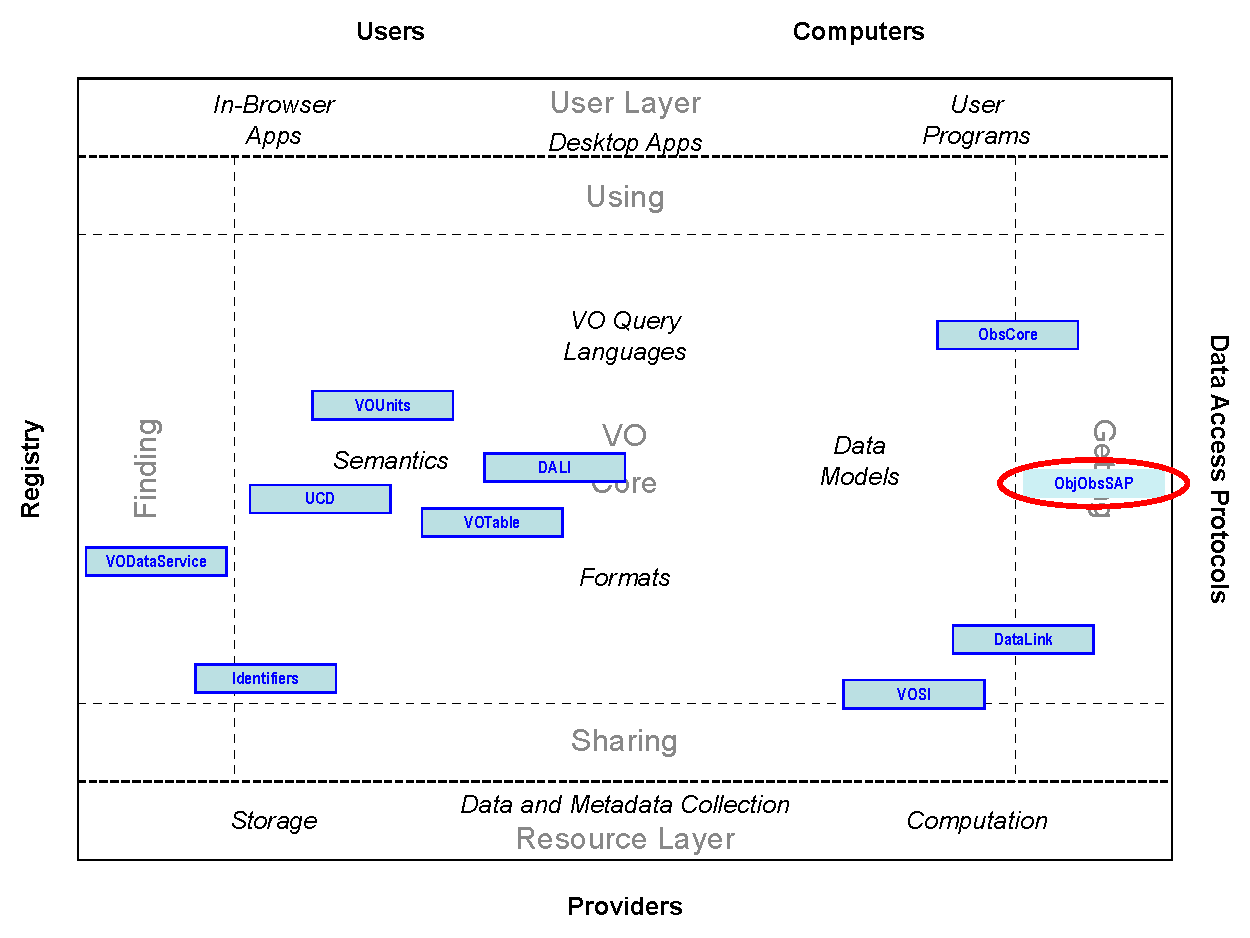
\includegraphics[width=6.0in,height=4.73in]{./role_diagram.pdf}
\end{figure}


%%%%%%%%%%%%%%%%%%%% Figure/Image No: 1 Ends here %%%%%%%%%%%%%%%%%%%%
\pagebreak



\section{Introduction}\label{section:_Toc415497365}


The Object Observability Simple Access Protocol (ObjObsSAP henceforth)
specifies in a standard format the services to retrieve object
observability from astronomical observatories.



The ObjObsSAP interface has intentionally been made similar to the SSAP
\citep{2012ivoa.spec.0210T} and SIAP v2.0 \citep{2015ivoa.spec.0617D} through the adoption
of current IVOA Data Access Layer Interface (DALI; \citealt{2017ivoa.spec.0517D}) and Observation Data
Model Core Components (ObsCore;\citealt{2017ivoa.spec.0509L}) and its implementation in
the Table Access Protocol (TAP;\citealt{2019ivoa.spec.0927D}). ObjObsSAP services also support
VOSI-availability and VOSI-capabilities resources (VOSI;\citealt{2017ivoa.spec.0524G}):



\begin{itemize}
\item queries encoded as URLs,
\item the use of VOTable for encoding search results,
\item the mechanism for handling errors, and
\item the retrieval of service metadata.
\end{itemize}


\subsection{The Role in the IVOA Architecture}
ObjObsSAP specifies standardID values \citep{2016ivoa.spec.0523D} for each
capability, as defined by VODataService \citep{2010ivoa.spec.1202P}. ObjObsSAP
services may be registered in an IVOA Registry using the SimpleDALRegExt
\citep{2017ivoa.spec.0530P} extension schema.


\section{Requirements for Compliance}
The object observability query web method \textbf{MUST} be supported as described
in section \ref{sec:query}. Through this web method, clients search for observability
periods based on given sky coordinates and a time period (optional). The
response is a VOTable that describes the constraint-free observability time
windows. Other output formats can be specified by the RESPONSEFORMAT
parameter (see \citet{2017ivoa.spec.0517D}).

\subsection{Compliance}
The keywords \textbf{MUST}, \textbf{REQUIRED}, \textbf{SHOULD},
and \textbf{MAY} as used in this document are to be interpreted as
described in RFC 2119.

An implementation is compliant if it satisfies all the \textbf{MUST}
or \textbf{REQUIRED} level requirements for the protocols it
implements. An implementation that satisfies all the \textbf{MUST} or
\textbf{REQUIRED} level and all the \textbf{SHOULD} level
requirements for its protocols is said to be "unconditionally
compliant"; one that satisfies all the \textbf{MUST} level
requirements but not all the \textbf{SHOULD} level requirements for
its protocols is said to be "conditionally compliant".

\section{Resources}
The purpose of the object observability query is to enable users and clients to
determine if a given set of sky coordinates is observable during a specified time period.
Here, "observable" refers to a time interval suitable for conducting scientific observations. 
The precise definition of when an object is deemed observable for scientific purposes is therefore left to the individual observatories.

The most basic query parameters will be the sky coordinates (Right
Ascension and Declination), both coordinates must be expressed following
the ICRS coordinate system and the start time and stop time for the
observability checks (optional). Any additional parameters may be used to
customize the observability checks.

The ObjObsSAP service have been designed to follow the DALI-sync
specification.

\begin{table}[h]
\centering
\begin{tabular}{|l|l|l|}
\hline
\textbf{resource type} & \textbf{resource name} & \textbf{required
} \\
\hline
\{query\} & service specific & yes \\
\hline
DALI-examples & /examples & no \\
\hline
VOSI-availability & /availability & yes \\
\hline
VOSI-capabilities & /capabilities & yes \\
\hline
\end{tabular}
\caption{ObjObsSAP service resources}
\end{table}
The ObjObsSAP service must have at least one \{query\} resource.

\subsection{\{query\} resource} \label{sec:query}
The \{query\} resource is a synchronous web service resource that
follows the DALI-sync description . The name and the path of the
resource is up to the implementer. The functionality to find the
resource path will be implemented using the VOSI-capabilities
resource.

As a DALI-sync resource, the parameters for a request may be submitted
using an HTTP GET (query string) or POST action.

Object observability services advertise their availability as described in
the DALI standard. This system must provide mechanisms to fully
characterize the service, including its non-compulsory and additional
parameters.

All parameters for the \{query\} resource are described below. Some of
these parameters are \textbf{MANDATORY }and others not, depending on
the astronomical facility characteristics. For example, \textbf{
elevation} input parameter may only be used for ground-based
observatories.

Parameters may appear in any order. If the same parameter appears
multiple times in a request, the operation is undefined (if alternate
values for a parameter are desired, the range-list syntax may be used
instead). Parameter names are case-insensitive. Parameter values are
case-sensitive unless defined otherwise in the description of an
individual parameter.

The following subsections define reserved parameters. In addition to the
description of the functional role the parameter plays in constraining a
query, each definition also includes, when applicable, a UCD and/or
UType that indicates the semantic meaning of the parameter. The UType
names refer to those defined in the ObsCore Data Model .

Some of the parameters proposed in this standard are not described in
the ObsCore Data Model document , such as; min\_obs, max\_obs,
elevation, moon\_sep. We tried to describe these parameters following
the ObsCore standard.

\subsubsection{Required parameters}
A service must support the input parameters described in this section.
That means that the service must accept them as valid ones without
raising an error, and the parameters must be properly used to constrain
the query.

As described in this section, the only mandatory parameters are the Right 
Ascension and Declination of the sky coordinates for checking constraint-free 
time intervals. In this context, the service will return all possible time 
intervals during which the sky coordinates are observable. The duration of 
these intervals will depend on the characteristics of each scientific 
instrument. For instance, ground-based optical telescopes typically cover 
longer observation periods than Low Earth Orbit observatories, where 
satellite orbital elements change frequently.


\begin{itemize}
\item{\textbf{MAXREC}\\MAXREC parameter is defined in DALI and allows
the client to limit the number or records in the response. A service
implementation may also impose default and maximum values for this limit.
However, the limit is determined, if the output is truncated due to the
limit the server must indicate this using an overflow (section 4.1)
indicator except in the special case of MAXREC=0, where the service
respond with metadata-only (normal output document with no records).}

\item{\textbf{UPLOAD}\\DALI UPLOAD parameter is not used by this version
of ObjObsSAP. The use case of uploading lists of coordinates is covered
by the multiple-valued parameters values.}

\item{\textbf{POS}\\The service \textbf{MUST }support the
\textbf{POS} parameter, to specify the position in the sky to check the observability. 
The coordinate values are specified in list format (comma separated) with no embedded white
space.\\
Example:\\
%%%%%%%%%%%%%%%%%%%% starts here %%%%%%%%%%%%%%%%%%%%
\begin{lstlisting}[language=SQL]
POS=52,-27.8
\end{lstlisting}
%%%%%%%%%%%%%%%%%%%% ends here %%%%%%%%%%%%%%%%%%%%
\par
POS defaults to right-ascension and declination in decimal degrees in
the ICRS coordinate system. This parameter has been defined in line with
other IVOA S*APs protocols although the optional coordinate system has
been removed for simplicity.}

\item{\textbf{TIME}\\The service \textbf{MUST} support the
\textbf{TIME} parameter, to specify the time coverage in range-list form
to check for object observability. The unit of \textbf{TIME} parameter must be
expressed in MJD. The format of the range list is the one defined by other
IVOA S*APs protocols like SSAP \citep{std:SSAP}, where the format of a
range is defined by '$t_{min}\slash t_{max}$'. If the range is defined
as an open range without the lower value of the range like '$\slash t_{max}$',
$t_{min}$ will be interpreted as now.\\

\textbf{Example:} to query for object observability of the coordinate
(10.68,41,27) and end time for the periods between 11-April-2021 and 
14-April-2021:
%%%%%%%%%%%%%%%%%%%% starts here %%%%%%%%%%%%%%%%%%%%
\begin{table}[h]
\centering
\begin{tabular}{|l|l|}
\hline
\begin{lstlisting}[language=SQL]
http://xmmvischeck.esac.esa.int:8080/objobssap/query?
POS=10.68,41.27&TIME=59522/59532
\end{lstlisting}
\\
\hline
\end{tabular}
\end{table}
%%%%%%%%%%%%%%%%%%%% ends here %%%%%%%%%%%%%%%%%%%%

Calculation of the observability by different observatories is only defined
for a certain future time range. That implies that there could be
\textbf{a maximum time hard limit} defined by the service that could be
smaller than the maximum of the \textbf{TIME} period value invoked by
the client. If this is the case, the information of the use of a maximum
time hard limit MAY be included in a certain $<$INFO$>$ VOTable tag in 
the service response like:
%%%%%%%%%%%%%%%%%%%% starts here %%%%%%%%%%%%%%%%%%%%
\begin{lstlisting}[language=SQL]
<INFO name="T_MAX_HARD_LIMIT" value="61231"/>
\end{lstlisting}
%%%%%%%%%%%%%%%%%%%% ends here %%%%%%%%%%%%%%%%%%%%
}
\end{itemize}

See \textit{Successful Response} section for more info about valid
VOTable res\-pon\-ses.

\subsubsection{Non-compulsory Parameters}
The next list of non-compulsory parameters may be implemented on the
server side. These parameters should be treated as reserved keywords.

\begin{itemize}
\item{\textbf{MIN\_OBS}\\A service \textbf{MAY} have a search parameter
called \textbf{MIN\_OBS}. This parameter would constrain the observability
check to those time periods with at least the minimum observability specified
in the parameter. The unit of \textbf{MIN\_OBS} parameters must be expressed
in seconds.\par
\textbf{Example:} The input parameter listing below from the Object
observability Simple Access Protocol shows that in addition to supporting
the required parameters (POS, TIME), it also supports the free
parameter MIN\_OBS.
%%%%%%%%%%%%%%%%%%%% starts here %%%%%%%%%%%%%%%%%%%%
\begin{lstlisting}[language=XML]
<?xml version="1.0" encoding="UTF-8"?>
<VOTABLE xmlns:xsi="http://www.w3.org/2001/XMLSchema-instance"
xsi:noNamespaceSchemaLocation="xmlns:http://www.ivoa.net/xml/
VOTable/VOTable-1.1.xsd"
xmlns:ovdm="http://www.ivoa.net/xml/ObjectObservabilityDM/
ObjectobservabilityDM-v1.0.xsd" version="1.0">
<RESOURCE type="results">
<DESCRIPTION>
Object Observability Simple Access Protocol
</DESCRIPTION>
<INFO name="QUERY_STATUS" value="OK"/>
<PARAM name="INPUT:POS" datatype="char" arraysize="*"
value="10.68">
<DESCRIPTION>
Specify the right ascension and declination coordinate.
To be specified in Equatorial Coordinates J2000.
</DESCRIPTION>
</PARAM>
<PARAM name="INPUT:TIME"
utype="Char.TimeAxis.Coverage.Bounds.Limits"
datatype="float"
unit="d" value="58171.45833/58321.958333">
<DESCRIPTION>
Specify the time coverage (epoch), specified in range-list form
to check for observability. To be specified in MJD.
</DESCRIPTION>
</PARAM>
<PARAM name="INPUT:MIN_OBS" ucd="time.duration"
utype="Char.TimeAxis.Coverage.Duration" unit="s"
datatype="float">
<DESCRIPTION> Minimum observability time interval
</DESCRIPTION>
</PARAM>
... ... ... ...
\end{lstlisting}
%%%%%%%%%%%%%%%%%%%% ends here %%%%%%%%%%%%%%%%%%%%

}
\item{\textbf{FACILITY}\\A service \textbf{MAY} have a search parameter
called \textbf{FACILITY}. This parameter would constrain the output of
observability ranges for services with multiple telescopes/facilities.
This could be used, e.g., to select observability ranges for telescopes
arrays, preventing the need of registration of one service per telescopes
for this kind of observatories. Also, this could be useful for antennas
arrays.}
\end{itemize}

\subsection{Availability: VOSI-availability}
A web service with ObjObsSAP capabilities  \citep{2017ivoa.spec.0524G} must have a
VOSI-availability resource as described in DALI \citep{2017ivoa.spec.0517D}.

\subsection{Capabilities: VOSI-capabilities}
A web service with ObjObsSAP capabilities must have a VOSI-capabilities
resource as described in DALI. The standardID for the \{query\}
capability is:

%%%%%%%%%%%%%%%%%%%% starts here %%%%%%%%%%%%%%%%%%%%
\begin{lstlisting}[language=SQL]
ivo://ivoa.net/std/ObjObsSAP#query-0.3
\end{lstlisting}
%%%%%%%%%%%%%%%%%%%% ends here %%%%%%%%%%%%%%%%%%%%
All DAL services must implement the /\textit{capabilities} resource.
The following capabilities document shows the minimal metadata and does
not require a registry extension schema:

%%%%%%%%%%%%%%%%%%%% starts here %%%%%%%%%%%%%%%%%%%%
\begin{lstlisting}[language=XML]
<?xml	version="1.0"	encoding="UTF-8"?>
<vosi:capabilities
 xmlns:vosi="http://www.ivoa.net/xml/VOSICapabilities/v1.0"
 xmlns:xsi="http://www.w3.org/2001/XMLSchema-instance"
 xmlns:vs="http://www.ivoa.net/xml/VODataService/v1.1">
 <capability standardID="ivo://ivoa.net/std/VOSI#capabilities">
  <interface xsi:type="vs:ParamHTTP" version="1.0">
   <accessURL use="base">
     http://example.com/ObjObsSAP/capabilities
   </accessURL>
  </interface>
 </capability>
 <capability standardID="ivo://ivoa.net/std/VOSI#availability">
  <interface xsi:type="vs:ParamHTTP" version="1.0">
   <accessURL	use="full">
    http://example.com/ObjObsSAP/availability
   </accessURL>
  </interface>
 </capability>
 <capability standardID="ivo://ivoa.net/std/ObjObsSAP#query-0.3">
  <interface xsi:type="vs:ParamHTTP" role="std"	version="0.3">
   <accessURL>
    http://example.com/ObjObsSAP/query
   </accessURL>
  </interface>
<!-- service details from extension schema could go here -->
 </capability>
</vosi:capabilities>

\end{lstlisting}
%%%%%%%%%%%%%%%%%%%% ends here %%%%%%%%%%%%%%%%%%%%

Note that the \{query\} resource does not have to be named as shown in
the access URL(s) above.

\section{\{query\} response}

\subsection{Successful Query}
The response from a successful call to the \{query\} resource is a
VOTable, or a different format following the RESPONSEFORMAT definition.
The ObsCore data model specifies all the VOTable \citep{2019ivoa.spec.1021O}
field names, utypes, UCDs, and units to use in the response, as well
as which fields must have values and which are allowed to be empty.\\
The \{query\} response must contain the required ObsCore \citep{2017ivoa.spec.0509L}
fields and may contain additional fields or custom fields from the service
provider. Examples are provided in Section 5.\par

Successfully executed requests should result in a response with HTTP
status code 200 (OK) and a response in the format requested by the
client or in the default format for the service. The default output
format is VOTable. Other output formats can be specified by the
RESPONSEFORMAT parameter \citep{2017ivoa.spec.0517D}.\par

The service should set the following HTTP headers to the correct values
where possible.

\begin{table}[h]
\centering
\begin{tabular}{|l|l|}
\hline
Content-Type & mime-type of the response \\
\hline
Content-Encoding & encoding/compression of the response (if applicable)
\\
\hline
\end{tabular}
\caption{Recommended HTTP Response Headers}
\end{table}
\par
Since the \{query\} response is usually dynamically generated, the
Content-Length and Last-Modified headers cannot usually be set.\\

The output returned by a ObjObsSAP service is a VOTable , an XML table
format, returned with a MIME-type of "application/x-votable+xml". The
table lists all the observability periods computed for the given
coordinates and time period in the server. The following requirements
are placed on the contents of the table when the query successfully
returns a list of observability periods:

\newcounter{numberedCntBI}
\begin{enumerate}
\item The VOTable \textbf{MUST} contain a RESOURCE element identified
with the tag type="results" should contain TABLE element which contains
the results of the query. The VOTable is permitted to contain additional
RESOURCE elements, but the usage of any such elements is not defined
here. If multiple resources are present it is recommended that the query
results be returned in the first resource element.
\item The RESOURCE element \textbf{MUST} contains an INFO element with
name="QUERY\_STATUS". Its value attribute should be set to "\,OK" if the
query executed successfully, regardless of whether any observability period
for the given coordinates were found.
\setcounter{numberedCntBI}{\theenumi}
\end{enumerate}

\textbf{Examples: }
%%%%%%%%%%%%%%%%%%%% starts here %%%%%%%%%%%%%%%%%%%%
\begin{lstlisting}[language=XML]

<INFO name="QUERY_STATUS" value="OK">
<INFO name="QUERY_STATUS" value="OK">Successful Checks</INFO>
\end{lstlisting}
%%%%%%%%%%%%%%%%%%%% ends here %%%%%%%%%%%%%%%%%%%%

\begin{enumerate}
\setcounter{enumi}{\thenumberedCntBI}
\item Each table row represents a different observability period.
\item Each record of the output VOTable \textbf{MUST} contain value
for each FIELD.
\item Every FIELD \textbf{SHOULD} contain a utype reference to the
object observability Data Model whenever possible.
\item A standard column \textbf{MUST} have a defined utype and a
defined UCD as described in next section
\item A standard column could appear multiple times with different
units. The way to uniquely identify one standard column is the
following:
\begin{itemize}
\item When a standard column can appear multiple times with the same
utype but different units, the column is uniquely identified by its
utype and unit.
\item Otherwise, a standard column is uniquely defined by its utype.
\end{itemize}
\item The VOTable \textbf{MUST} contain a reference to the OVDM
namespace
\setcounter{numberedCntBI}{\theenumi}
\end{enumerate}

%%%%%%%%%%%%%%%%%%%% starts here %%%%%%%%%%%%%%%%%%%%
\begin{lstlisting}[language=XML]
xmlns:ovdm="http://www.ivoa.net/xml/ObjectObservabilityDM/
ObjectObservabilityDM-v1.0.xsd"
\end{lstlisting}
%%%%%%%%%%%%%%%%%%%% ends here %%%%%%%%%%%%%%%%%%%%

\subsubsection{Standard output fields}
A detailed reference of the data model can be found in Appendix A

\begin{itemize}
\item {Exactly one field \textbf{MUST} have a name="\textbf{t\_validity}"
with\\ utype=" \textbf{Char.TimeAxis.Coverage.Time}" with
datatype="float", ucd="time.validity", unit="d" containing the date when the observability calculations will change.}

\item {Exactly one field \textbf{MAY} have a name="\textbf{validity\_accuracy}" 
with datatype="char" and arraysize="*" containing the level of
confidence of the validity range, with one of the following allowed
values: HIGH, MEDIUM, LOW.}

\item {Exactly one field \textbf{MAY} have a name="\textbf{
validity\_predictor}" with datatype="char" and arraysize="*" with an
identifier of the software used to calculate the observability.}

\item {Exactly one field \textbf{MUST} have a name="\textbf{t\_start}" with\\
utype="\textbf{Char.TimeAxis.Coverage.Bounds.Limits.StartTime}"\\ with
datatype="float",  ucd="time.start", unit="d" containing the start of the observability period.}

\item {Exactly one field \textbf{MUST} have a name="\textbf{t\_stop}" with\\
utype="\textbf{Char.TimeAxis.Coverage.Bounds.Limits.StopTime}"\\, with
datatype="float", ucd="time.end" and unit="d" containing the end of the observability period.}

\item {Exactly one field \textbf{MUST} have a name="\textbf{t\_observability}"
with\\ utype="\textbf{Char.TimeAxis.Coverage.Support.Extent}"\\, with
datatype="float", ucd="time.duration" and unit="s", containing the observability window duration in seconds.}

\item {Exactly one field \textbf{MAY }have a name="\textbf{pos\_angle
}" with\\
utype="\textbf{Char.SpatialAxis.Coverage.Location.Coord.Position2D.Value2.C3}"\\
datatype="float", ucd="pos.eq.pos\_angle" and
unit="deg", containing the spacecraft position angle.}

\item {Exactly one field \textbf{MAY }have a name="\textbf{em\_min}" with\\
utype="\textbf{Char.Spectral.Axis.Energy.Min}"\\
datatype="float", ucd="em.energy" and unit="m" , containing the low energy bound for this particular sky position and observability time interval.}

\item {Exactly one field \textbf{MAY }have a name="\textbf{em\_max}" with\\
utype="\textbf{Char.Spectral.Axis.Energy.Max}"\\
datatype="float", ucd="em.energy" and unit="m" , containing the high energy bound for this particular sky position and observability time interval.}

\item {Exactly one field \textbf{MAY }have a name="\textbf{max\_obs}" with\\
utype="\textbf{Char.TimeAxis.Coverage.Support.Extent}"\\ with 
datatype="float", ucd="time.duration" and unit="s" , containing the maximum observavility period for the given sky position at the given time.} 

\item {Exactly one field \textbf{MAY }have a name="\textbf{elevation\_min}" with\\
utype="\textbf{Char.Position.Axis.Min}"\\ with
datatype="float", ucd="angle.validity" and unit="deg" , containing the minimum elevation for this particular sky position and observability time interval.}

\item {Exactly one field \textbf{MAY }have a name="\textbf{elevation\_max}" with\\
utype="\textbf{Char.Position.Axis.Max}"\\
datatype="float", ucd="angle.validity" and unit="deg", containing the maximum elevation for this particular sky position and 
observability time interval.}

\item {Exactly one field \textbf{MAY }have a name="\textbf{moon\_sep\_min}" 
datatype="float", ucd="angle.validity" and
unit="deg" , containing the minimum Moon separation for this particular
sky position and observability time interval.}

\item {Exactly one field \textbf{MAY }have a name="\textbf{moon\_sep\_max}" 
datatype="float", ucd="angle.validity" and
unit="deg" , containing the maximum Moon separation for this particular
sky position and observability time interval.}

\item {Exactly one field \textbf{MAY }have a name="\textbf{sun\_sep\_min}" with\\
datatype="float", ucd="angle.validity" and
unit="deg" , containing the minimum Sun separation for this particular
sky position and observability time interval.}

\item {Exactly one field \textbf{MAY }have a name="\textbf{sun\_sep\_max}" with\\
datatype="float", ucd="angle.validity" and
unit="deg" , containing the maximum Sun separation for this particular
sky position and observability time interval.}

\item {Exactly one field \textbf{MAY} have a name="\textbf{facility}" 
with datatype="char" and arraysize="*", ucd="meta.id;instr.tel",\\
utype="\textbf{Provenance.ObsConfig.Facility.name}",\\ 
containing the identifier of the telescope/antenna/facility to which
this range period is applicable. The value could be a data provider
defined shortname for the facility. \\
Examples: HST/WFPC2, VLT/FORS2, SKA1/LOW11, etc}
\end{itemize}

\subsubsection{ObjObsSAP \{query\} Service Descriptor}
The DataLink specification describes a mechanism for describing a
service within a VOTable resource and recommends that services can
describe themselves with a special resource with name="this". ObjObsSAP
\{query\} responses should include a descriptor describing both standard
and custom query parameters (if applicable). The descriptor for a
service with standard parameters (see 3.1) would be:\\

%%%%%%%%%%%%%%%%%%%% starts here %%%%%%%%%%%%%%%%%%%%
\begin{lstlisting}[language=XML]
<RESOURCE type="meta" utype="adhoc:service" name="this">
<PARAM name="standardID" datatype="char" arraysize="*"
    value="ivo://ivoa.net/std/ObjObsSAP#query-0.3"/>
<PARAM name="accessURL" datatype="char" arraysize="*"
    value="http://example.com/ObjObsSAP/query"/>
 <GROUP name="inputParams">
  <PARAM name="pos" datatype="char" arraysize="*"/>
  <PARAM name="time" datatype="float" arraysize="*"	 unit="d"/>
  <PARAM name="min_obs" datatype="float" arraysize="*"	unit="s"/>
 </GROUP>
</RESOURCE>
\end{lstlisting}
%%%%%%%%%%%%%%%%%%%% ends here %%%%%%%%%%%%%%%%%%%%

This VOTable resource should be included in the output from all queries;
it is especially useful for MAXREC=0 queries since inclusion of the
self-descriptor would mean that all inputs and outputs would be fully
described

\section{Output Example}
%%%%%%%%%%%%%%%%%%%% starts here %%%%%%%%%%%%%%%%%%%%
\begin{lstlisting}[language=SQL]
<?xml version="1.0" encoding="UTF-8"?>
<VOTABLE xmlns:xsi="http://www.w3.org/2001/XMLSchema-instance"
xsi:noNamespaceSchemaLocation="
xmlns:http://www.ivoa.net/xml/VOTable/VOTable-1.1.xsd"
xmlns:ssldm="http://www.ivoa.net/xml/
ObjectObservabilityDM/ObjectObservabilityDM-v1.0.xsd"
version="1.0">
<RESOURCE type="results">
<DESCRIPTION>
European Space Astronomy Centre. XMM-Newton SOC -
Object Observability Simple Access Protocol (ObjObsSAP)
</DESCRIPTION>
<INFO name="QUERY_STATUS" value="OK"/>
<INFO name="SERVICE PROTOCOL" value="1.0">
ObjObsSAP
</INFO>
<INFO name="POS" value="10.68,41.27"/>
<INFO name="TIME" value="58171.45833/58321.958333"/>
<TABLE>
<FIELD name="t_start" ucd="time.start"
utype="Char.TimeAxis.Coverage.Bounds.Limits.StartTime"
datatype="float" unit="s"/>
<FIELD name="t_stop" ucd="time.end"
utype="Char.TimeAxis.Coverage.Bounds.Limits.StopTime"
datatype="float" unit="s"/>
<FIELD name="t_observability"
utype="Char.TimeAxis.Coverage.Support.Extent"
ucd="time.duration" datatype="float" unit="s"/>
<DATA>
<TABLEDATA>
<TR>
<TD>58297.123611</TD>
<TD>58297.436806</TD>
<TD>27036</TD>
</TR>
<TR>
<TD>58298.534028</TD>
<TD>58299.438194</TD>
<TD>78126</TD>
</TR>
... more lines data ...
</TABLEDATA>
</DATA>
</TABLE>
</RESOURCE>
</VOTABLE>
\end{lstlisting}
%%%%%%%%%%%%%%%%%%%% ends here %%%%%%%%%%%%%%%%%%%%
\bibliography{ivoatex/ivoabib,ivoatex/docrepo.bib}
\appendix
\renewcommand{\thesection}{\Alph{section}.\arabic{section}}
\setcounter{section}{0}
\begin{appendices}
\section{ObjObsSAP data model summary}
\FloatBarrier
\begin{table}[h]
\tiny
\centering
\begin{adjustbox}{angle=90}
\begin{tabular}{|p{25mm}|p{50mm}|p{20mm}|p{40mm}|p{15mm}|p{10mm}|}
\hline
Name & UTYPE & UCD & Description & DataType & Unit \\
\hline
\textbf{t\_validity} & \textbf{Char.TimeAxis.Coverage.Time  \newline
(MUST)} &
time.validity & Date when the \newline
observability calculation will change (MJD) &
float & d \\
\hline
\textbf{validity\_accuracy} & \textbf{(MAY)} & & Level of confidence
of the validity range \newline
Accepted values= HIGH, MEDIUM, LOW & char, * & \\
\hline
\textbf{validity\_predictor} & \textbf{(MAY)} & & Identifier (string
free representation) of the software used to calculate the observability &
char, * & \\
\hline
\textbf{t\_start} & \textbf{
Char.TimeAxis.Coverage.Bounds. \newline
Limits.StartTime  \newline
(MUST)} & time.start &
observability window start time (MJD) & float & d \\
\hline
\textbf{t\_stop} & \textbf{
Char.TimeAxis.Coverage.Bounds. \newline
Limits.StopTime \newline
(MUST)} & time.end &
observability widow end time (MJD) & float & d \\
\hline
\textbf{t\_observability} & \textbf{
Char.TimeAxis.Coverage. \newline
Support.Extent  \newline
(MUST)} & time.duration &
observability duration window & float & s \\
\hline
\textbf{pos\_angle} & \textbf{
Char.SpatialAxis.Coverage.Location. \newline
Coord.Position2D.Value2.C3  \newline
(MAY)} &
pos.eq.pos\_angle & Satellite position angle & float & deg \\
\hline
\textbf{em\_threshold} & \textbf{
Char.Spectral.Axis.Energy.Threshold \newline
(MAY)} & em.energy & Energy
threshold for this particular sky position and observability time interval
& float & m \\
\hline
\pagebreak
\textbf{target\_name} & \textbf{Target.Name  \newline
(MAY)} & meta.id;src &
Target Name & string & unitless \\
\hline
\textbf{em\_min} & \textbf{Char.Spectral.Axis.Energy.Min \newline
(MAY)} &
em.energy & Energy minimum for this particular sky position and
observability time interval & float & m \\
\hline
\textbf{em\_max} & \textbf{Char.Spectral.Axis.Energy.Max \newline
(MAY)} &
em.energy & Energy maximum for this particular sky position and
observability time interval & float & m \\
\hline
\textbf{elevation\_min} & \textbf{
Char.SpatialAxis.Coverage. \newline
Extent.angular\_distance \newline
(MAY)} & phys.angDist
& Minimum elevation for this sky position and observability time interval &
float & deg \\
\hline
\textbf{elevation\_max} & \textbf{
Char.SpatialAxis.Coverage. \newline
Extent.angular\_distance \newline
(MAY)} & phys.angDist
& Maximum elevation for this sky position and observability time interval &
float & deg \\
\hline
\textbf{moon\_sep\_min} & \textbf{(MAY)} & phys.angDist & Minimum
Moon separation for this sky position and observability time interval &
float & deg \\
\hline
\textbf{moon\_sep\_max} & \textbf{(MAY)} & phys.angDist & Maximum
Moon separation for this sky position and observability time interval &
float & deg \\
\hline
\textbf{sun\_sep\_min} & \textbf{(MAY)} & phys.angDist & Minimum Sun
separation for this sky position and observability time interval & float &
deg \\
\hline
\textbf{sun\_sep\_max} & \textbf{(MAY)} & phys.angDist & Maximum Sun
separation for this sky position and observability time interval & float &
deg \\
\hline
\textbf{facility} & \textbf{Char.SpatialAxis.Coverage.Provenance.\newline ObsConfig.Facility.name} 
\newline
\textbf{(MAY)} & meta.id;instr.tel & Identifier of the 
telescope/antenna/facility to which this range period is applicable 
& string & \\
\hline
\end{tabular}
\end{adjustbox}
\end{table}
\FloatBarrier

\section{Changes from Previous Versions}

\begin{table}[h]

\begin{tabularx}{\linewidth}{|L|c|l|}
\hline
\textbf{Change} & \textbf{Section} & \textbf{Version} \\
\hline
Visibility concept has been replaced by observability & all & WD-20241027 \\
\hline
min\_vis and max\_vis parameters have been replaced by 
min\_obs and max\_obs, respectively & all  & WD-20241027 \\
\hline
t\_visibility column changed by t\_observability & all & WD-20241027 \\
\hline
\end{tabularx}
\end{table}


\end{appendices}
\end{document}
